\documentclass[crop=false, class=book]{standalone}

%pacchetto per immagini
\usepackage{graphicx}
\usepackage{subfig}

\usepackage[italian]{varioref}
\usepackage{copyrightbox}
\usepackage{url}

\usepackage{enumitem}
\newcommand\litem[1]{\item{\bfseries #1:}}


\begin{document}
	\chapter{Cloud Anchors}
	L'API ARCore \textit{Cloud Anchor} introduce i cloud anchor, un tipo speciale di anchor che permettono di condividere con altri utenti l'esperienza AR. In particolare, un dispositivo può posizionare oggetti virtuali nello spazio, e altri utenti possono vedere l'oggetto virtuale ed interagire con esso trovandosi nella stessa posizione, come spiegato da \cite{kert2021mobile}.
	\\
	Questo tipo di anchor, come spiegato dalla documentazione ufficiale \cite{google2022cloud}, trova applicazione ad esempio per creare oggetti virtuali che persistano nel mondo reale, cioè che mantengano nel tempo la posizione in cui sono stati creati, oppure per creare giochi virtuali multigiocatore in cui è importante la collaborazione tra utenti in tempo reale.
	
	\section{Funzionamento}
	La creazione e la diffusione dell'anchor avviene tramite connessione internet in quattro passaggi, descritti ad alto livello come segue. La figura~\vref{fig:cloud} tratta dalla guida ufficiale Google descrive visivamente le quattro fasi del funzionamento dei cloud anchor.
	\begin{enumerate}
		\litem{Creation} l'utente crea un anchor localmente;
		\litem{Hosting} ARCore carica i dati della mappa 3D dello spazio circostante all'anchor locale nell'ARCore Cloud Anchor, che a sua volta restituisce al dispositivo un Cloud Anchor ID univoco;
		\litem{Distribution} l'app distribuisce l'ID univoco agli altri utenti;
		\litem{Resolving} gli utenti possono utilizzare l'ID ricevuto per ricreare l'anchor quando si trovano nello stesso ambiente. L'API compara la scena del dispositivo con la mappa 3D caricata precedentemente per determinare la posizione dell'utente e visualizzare correttamente l'oggetto virtuale.
	\end{enumerate}
	
	\begin{figure}[t]
		\centering
		\subfloat[][\emph{Creazione dell'anchor locale.}]
		{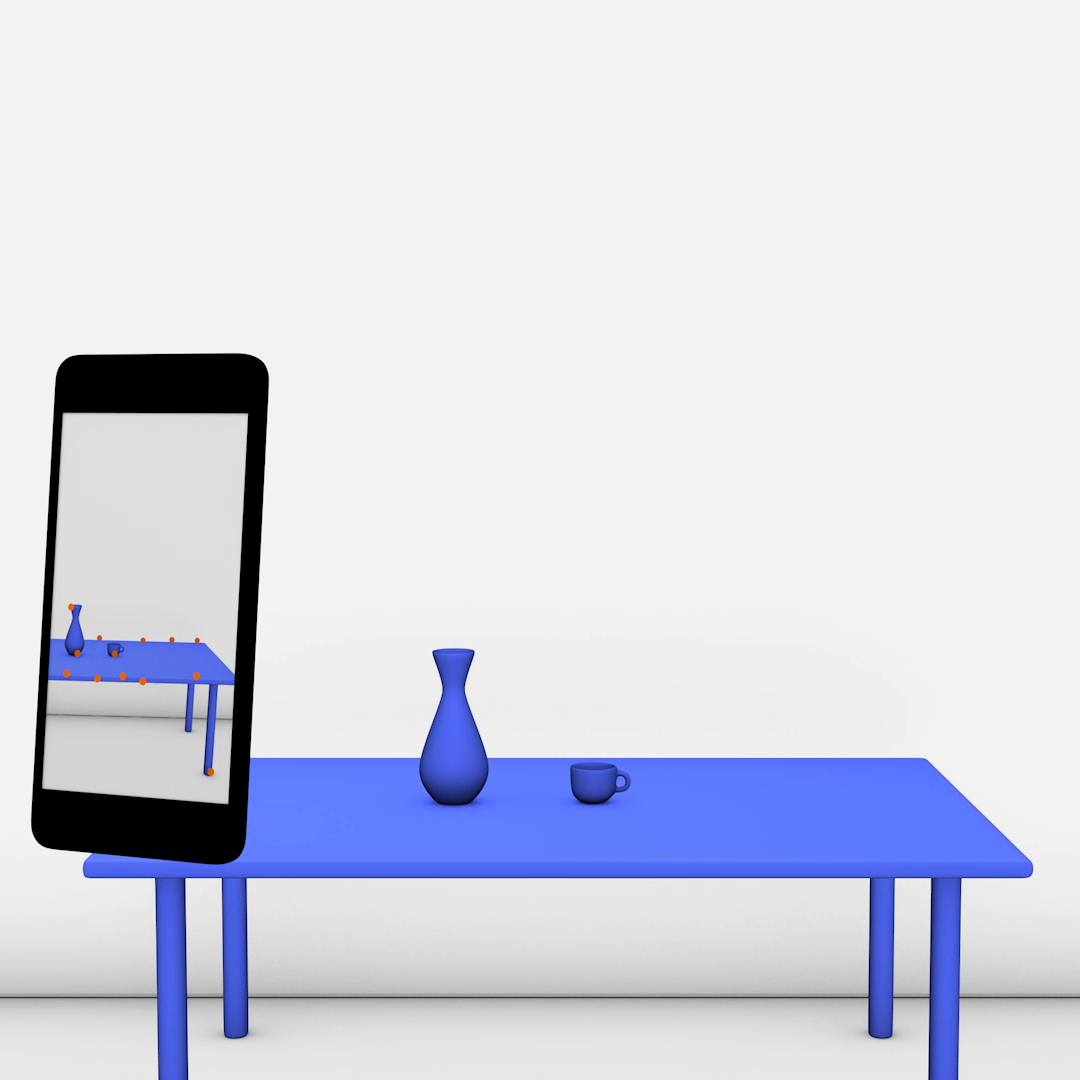
\includegraphics[width=0.45\textwidth]{./resources/images/cloud_anchors/creation}}  \quad
		\subfloat[][\emph{Hosting dell'anchor.}]
		{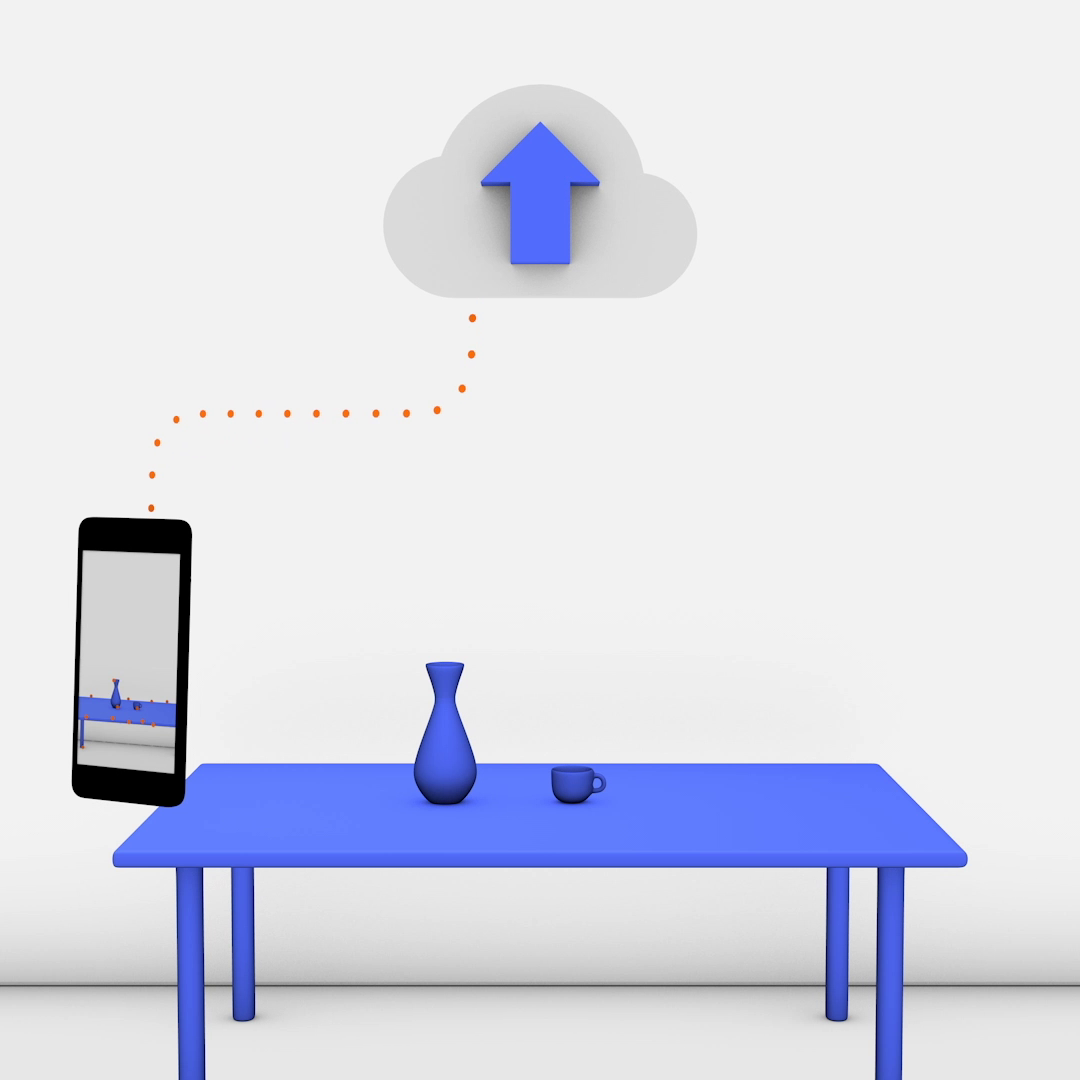
\includegraphics[width=0.45\textwidth]{./resources/images/cloud_anchors/hosting}} \\
		\subfloat[][\emph{Richiesta resolve al cloud anchor.}]
		{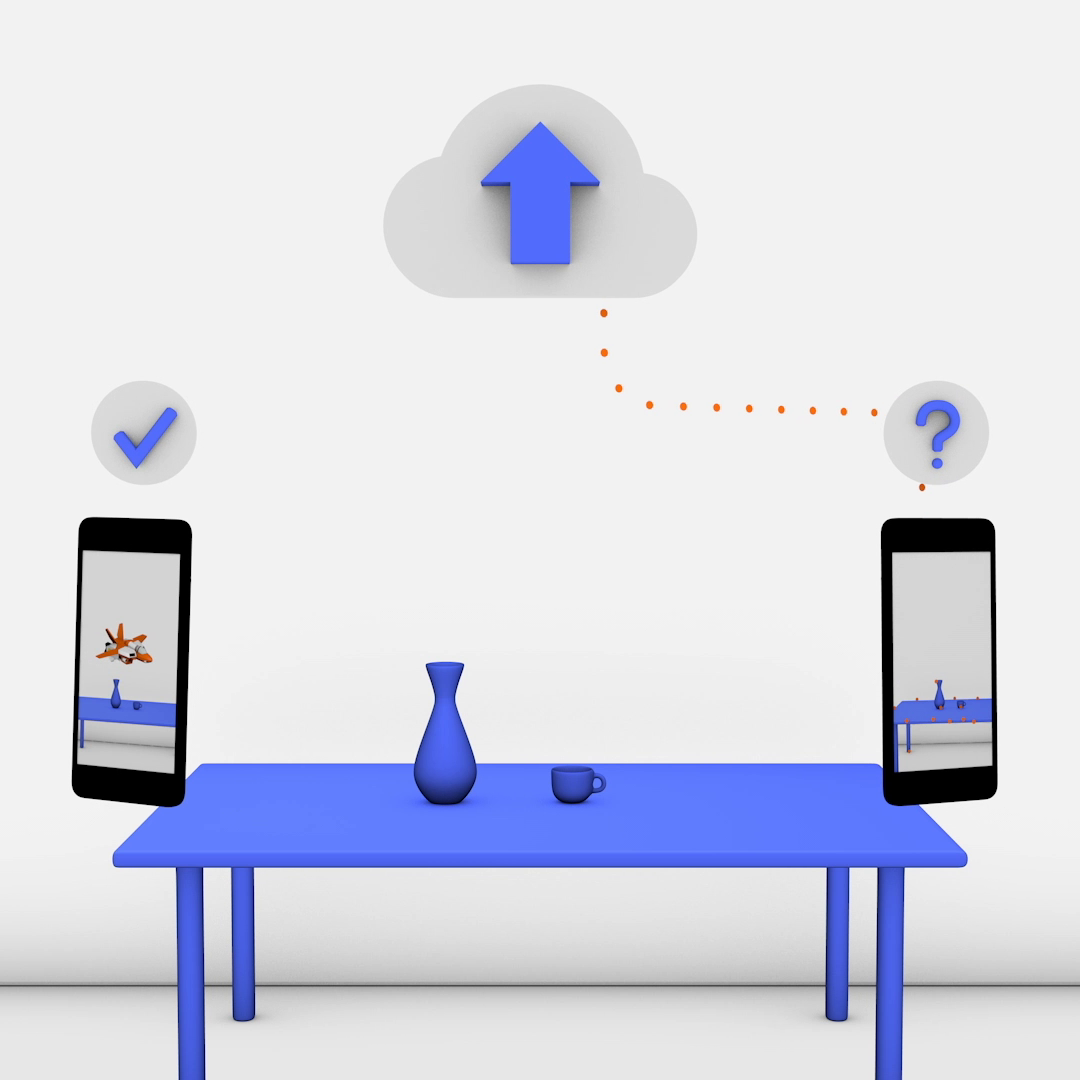
\includegraphics[width=0.45\textwidth]{./resources/images/cloud_anchors/distribution}} \quad
		\subfloat[][\emph{Resolve del cloud anchor.}]
		{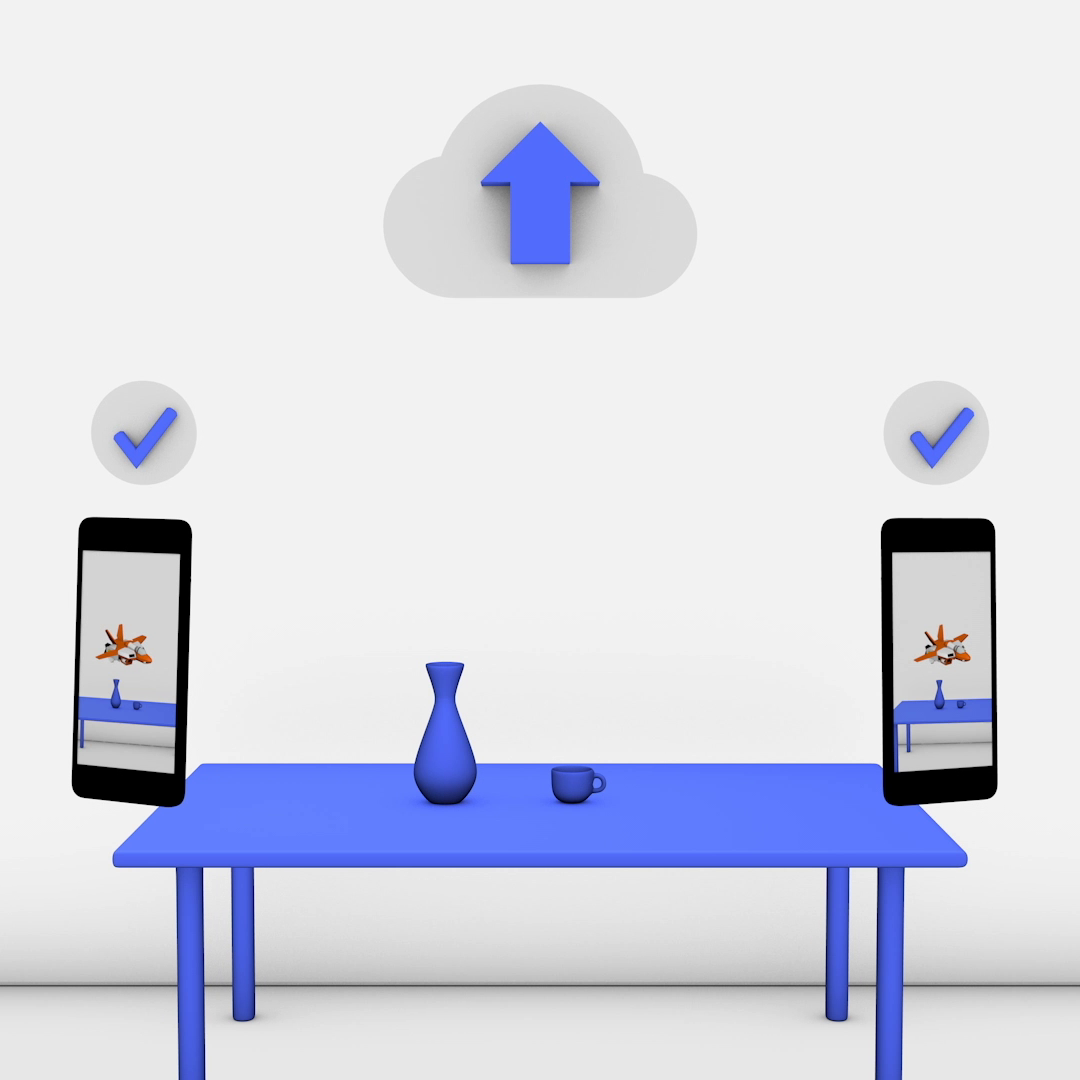
\includegraphics[width=0.45\textwidth]{./resources/images/cloud_anchors/resolving}}
		\caption{Funzionamento ad alto livello di Cloud Anchor API.}
		\label{fig:cloud}
	\end{figure}

	\section{Configurazione e utilizzo}
	Per implementare un'applicazione che utilizzi i Cloud Anchor è prima necessario creare un progetto in \textit{Google Cloud Platform} e abilitare il ARCore Cloud Anchor API per l'hosting, il salvataggio e il resolving degli anchor.
	\\
	\noindent
	La sessione ARCore deve essere impostata per poter utilizzare l'API Cloud Anchors, come descritto dal listing~\vref{lst:ca_session} tratto dalla documentazione ufficiale.
	\begin{center}
		\begin{minipage}{0.95\textwidth}
			\begin{lstlisting}[caption={Configurazione della modalità Cloud Anchor.}, label={lst:ca_session}, language=Kotlin]
			val config = Config(session)
			config.cloudAnchorMode = Config.CloudAnchorMode.ENABLED
			session.configure(config)
			\end{lstlisting}
		\end{minipage}
	\end{center}

	\subsection{Autenticazione}
	\label{subsec:auth}
	Se il cloud anchor deve poter avere processi host/resolve di durata massima 24 ore, come ad esempio per giochi virtuali multigiocatore, è necessaria un'autenticazione tramite chiave dell'app. Tale autenticazione si compie generando una \textit{API key} per il progetto cloud dal \textit{Google Cloud Console} e aggiungendola nel campo \verb|android:value| in un tag \verb|meta-data|, nel campo \verb|application| del file \verb|AndroidManifest.xml| dell'applicazione, come spiegato dal listing~\vref{lst:auth}.
	\begin{center}
		\begin{minipage}{0.95\textwidth}
			\begin{lstlisting}[caption={Autenticazione con API key.}, label={lst:auth}, language=xml, morekeywords={android:name, android:value}, keywordstyle={\color{NavyBlue}\bfseries}, alsodigit={-}, stringstyle={\color{ForestGreen}\ttfamily}, emph={meta-data},emphstyle={\color{OrangeRed}}]
			<meta-data
				android:name = "com.google.android.ar.API_KEY"
				android:value = "API_KEY"/>
			\end{lstlisting}
		\end{minipage}
	\end{center}

	\noindent
	Per cloud anchor che devono persistere per una durata compresa tra 1 e 365 giorni invece, è necessaria un'autenticazione tramite \textit{OAuth client}, che associa l'applicazione android al progetto di Google Cloud Platform. Tale autenticazione richiede una chiave \textit{SHA-1 fingerprint} che si può generare con il task \verb|signingReport| di Gradle.
	
	\subsection{Hosting}
	Il metodo \verb|hostCloudAnchorWithTtl(anchor:Anchor, ttlDays:Int)| della classe \verb|Session| permette di iniziare l'hosting di \verb|anchor| con una durata di \verb|ttlDays| giorni, un numero positivo compreso tra 1 e 365; per hosting con durata fino a 24 ore è invece necessaria l'invocazione del metodo \verb|hostCloudAnchor(anchor:Anchor)|. Entrambi i metodi restituiscono il nuovo anchor, con la stessa posizione di \verb|anchor| e con stato \verb|Anchor.CloudAnchorState.TASK_IN_PROGRESS|. Il listing~\vref{lst:hosting} tratto dal codelab \cite{codelab2021cloud} realizza l'hosting tramite un oggetto della classe wrapper \verb|CloudAnchorManager|.
	
	\begin{center}
		\begin{minipage}{0.95\textwidth}
			\begin{lstlisting}[caption={Hosting di un cloud anchor.}, label={lst:hosting}, language=Kotlin]
			val cloudAnchorManager : CloudAnchorManager = CloudAnchorManager();
				
			// Realizza l'hosting per l'anchor currentAnchor con durata 300 giorni
			cloudAnchorManager.hostCloudAnchor(session,currentAnchor,300,this::onHostedAnchorAvailable);
			\end{lstlisting}
		\end{minipage}
	\end{center}
	
	\subsection{Resolving}
	Il metodo \verb|resolveCloudAnchor(String cloudAnchorId)| della classe \verb|Session| compie il resolving, creando un anchor sulla base delle informazioni 3D inviate e comparate con la mappa 3D caricata durante l'hosting, per poter posizionare correttamente l'oggetto rispetto al dispositivo che sta compiendo il resolving.

	
\end{document}